\documentclass[10pt]{article}
\newcommand{\HRule}{\rule{\linewidth}{0.5mm}}
\parindent 0pt
\parskip 10pt
\usepackage{anysize}
\usepackage{graphicx}
\usepackage{epsfig}
\usepackage{float}
%\usepackage{cite}
\usepackage{natbib}
\usepackage{setspace}
\marginsize{3.5cm}{3.5cm}{1cm}{1cm}
\onehalfspacing
\usepackage{caption}
\usepackage{subcaption}
\usepackage{amsmath,hyperref}

\usepackage{xcolor}
\hypersetup{
    colorlinks,
    linkcolor={red!50!black},
    citecolor={blue!50!black},
    urlcolor={blue!80!black}
}

%\textwidth 15cm
%\textheight 24cm
%\onehalfspacing
\begin{document}

\title{Machine Learning Study: Breast Cancer Survivability Projections}

\author{David Starkey}

\maketitle





\section{Breast Cancer Machine Learning Study}
In the following short study, I use a variety of machine learning techniques to classify the recurrence probability of breast cancer as a function of a XX input characteristics (variables). Breast cancer is the most commonly diagnosed cancer in women and the second leading cause of cancer death among women in the UK. In the following study

 I aim to:

\begin{itemize}
\item Compare the relative computation time and accuracy between a three-layer neural network with five neurons in the hidden layer, and a k-nearest neighbour algorithm

\item Investigate whether the computation efficiency of the two algorithms can be improved by first using principal component analysis (PCA) to reduce the dimensionality of the parameter space, and determine the extent to which this can be achieved without compromising the classification accuracy. 

\end{itemize}



\section{Data Source}
The output data set is described in \href{ https://archive.ics.uci.edu/ml/datasets/Breast+Cancer
}{\textcolor{blue}{https://archive.ics.uci.edu/ml/datasets/Breast+Cancer
}} and classifies whether breast cancer is likely or unlikely to recur as a function of the input attributes. These include age of first diagnosis, tumour size etc. Here, two machine learning approaches are compared to investigate which is most efficient and accurate at predicting a recurrence of the disease.

\section{K-nearest neighbour algorithm and classification}
The first machine learning method used to classify the breast cancer data is known as k-nearest-neighbour. The algorithm can be summarised as follows:

\begin{itemize}
\item for each example $\vec{X_i}$ in the test dataset, calculate the euclidean distance to every $j$th point $\vec{y_j}$ in the training sample. For an $l$ dimensional dataset, this is 
\begin{equation}
d_{ij} = \sqrt{\left( \sum_l X_{il} - y_{jl} \right)^2}.
\label{eq_euclid}
\end{equation}

\item From the above quantities, identify the k ($k = 3$ is chosen for this work) closest points to data point $\vec{X_i}$ and calculate the mode classification of these $k$ closest points in the training set.

\item assign this classification to the test point $\vec{X_i}$ and repeat for the remaining examples.


\end{itemize}


K-nearest-neighbour is a simple but robust machine learning classification algorithm. One can avoid over-fitting to noise in the training data by choosing a suitably large value of k such that a rogue point in the training data is down weighted by the remaining of the $k-1$ points adjacent to $\vec{X_i}$ when calculating the mode classification.








\section{Hidden-Layer Neural Network}

Neural networks are slightly more difficult algorithms to understand theoretically but have the advantage that, once trained on a training sample, are faster at classifying new test examples than a K-nearest neighbour method.  The section below will outline the theory of a single layer neural network before developing this to a neural network with a hidden layer. The interested reader is advised to consult XX that offers an excellent in-depth discussion of the required, linear algebra, calculus and statistics involved in all steps of the back propagation algorithm used to train a neural network.

\subsection{Theory} 


In its simplest form, a neural network is composed of a single ($j=1$) `neuron'. This neuron takes an arbitrary number of $i$ input values, each modulated by a `weight' parameter $W_{ij}$ \footnote{Much of the theory in this section can be found in most texts on neural networks but wikipedia does a good job explaining the mathematical detail \href{ https://en.wikipedia.org/wiki/Backpropagation}{\textcolor{blue}{https://en.wikipedia.org/wiki/Backpropagation}}, as do the online Stanford lecture series' \href{ https://www.coursera.org/lecture/machine-learning/backpropagation-algorithm-1z9WW}{\textcolor{blue}{https://www.coursera.org/lecture/machine-learning/backpropagation-algorithm-1z9WW}}}. The weighted sum of these is known as the `activation' $z$ and is operated on by the neuron with an activation function $f (z)$ to yield an output quantity $a$. The output from the entire neural network for an input data example vector $\vec{X}_n$ (in situations with a chain of neurons as is the case later) is denoted $h(W,\vec{X}_n)$. A back propagation approach is used to optimize the weights (detailed below) in multi layer neural networks. This requires that the activation function $f(z)$ be differentiable. In this project (as is common for many neural networks), a sigmoid activation function is adopted where 

\begin{equation} 
f(z) = \frac{1}{1+e^{-z}},
\label{eq_sigmoid}
\end{equation}

\noindent with a derivative

\begin{equation} 
f`(z) = f(z) \left( 1 - f(z) \right).
\label{eq_sigmoid}
\end{equation}


\noindent This activation function always returns a number between 0 and 1. Once the weights are optimised, the neuron will output a value close to 0 to indicate one class, and close to 1 to indicate the other. The mathematical rigour in neural networks is in the weight-optimisation step. 


\begin{figure}
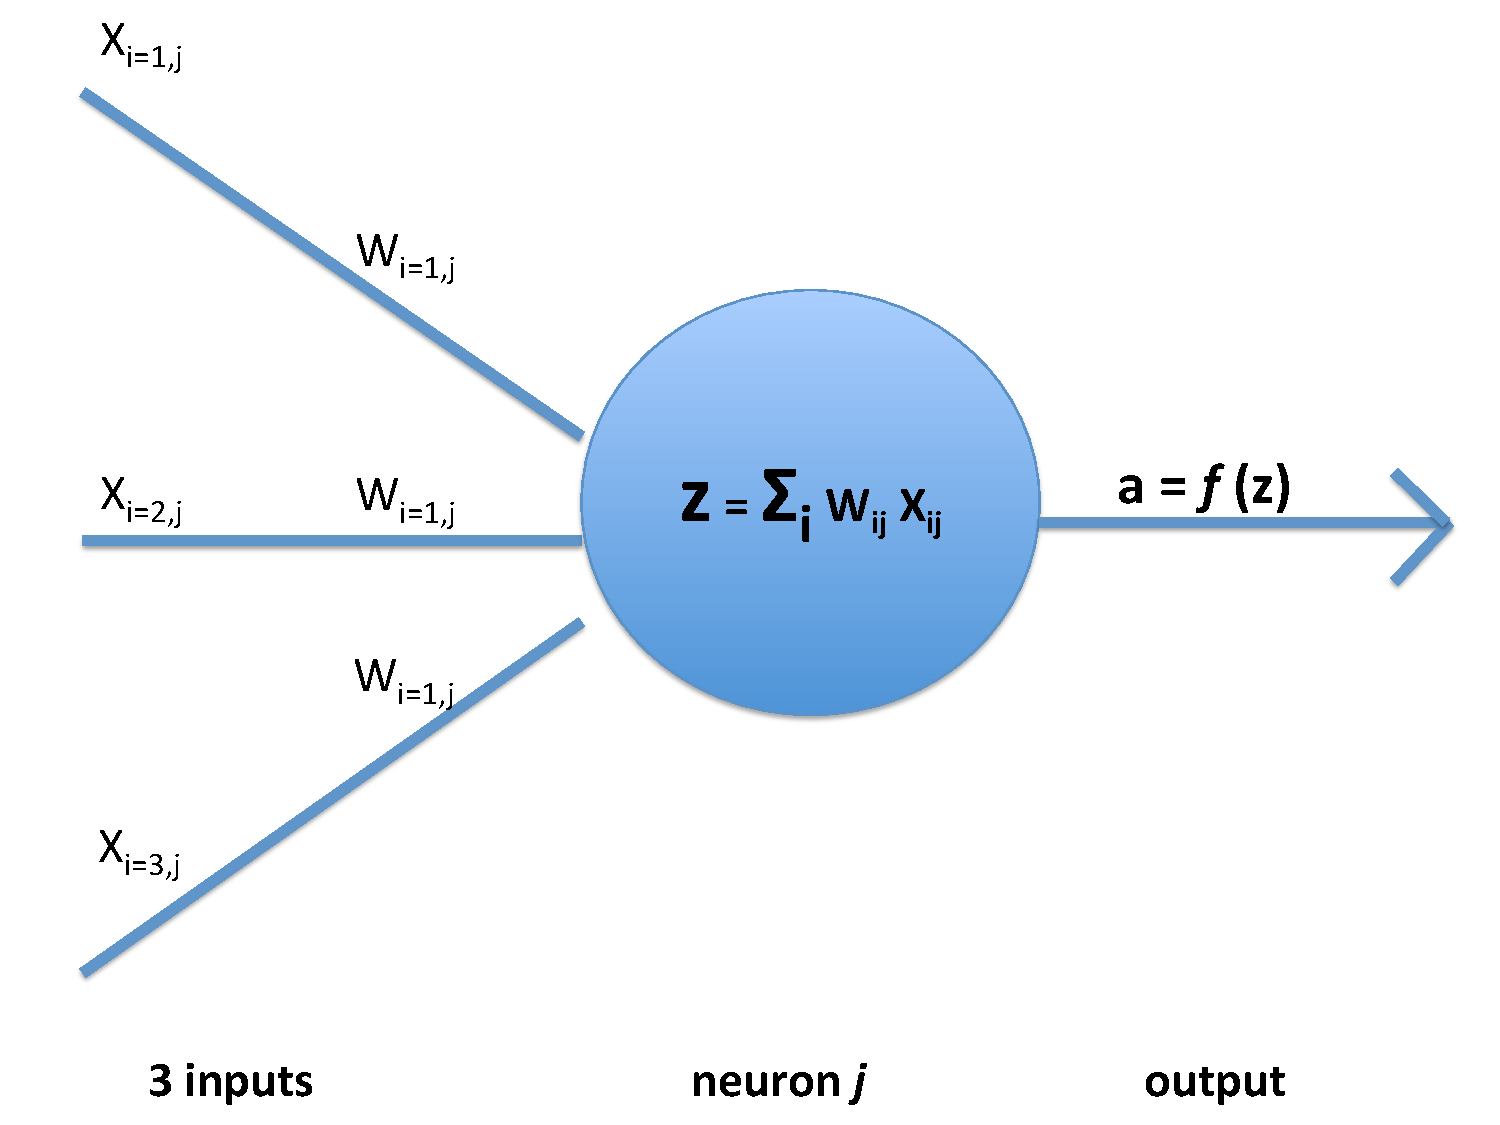
\includegraphics[scale=0.5,angle=0,trim=0cm 0cm 0.0cm 0cm]{diagrams.pdf}
\caption{Example neural network with a single neuron. The network has three inputs to neuron $j$ denoted by $X_{ij}$ with weights $W_{ij}$. The output from the neuron is given by $a_j$ where the activation function $f(z)$ is given in Equation \ref{eq_sigmoid}.}
\label{fig_temp}
\end{figure}


\subsection{optimizing the weights}

Like many optimisation problems, I start with the cost function (often called $\chi^2$ or the error function). For a single (or multi) layer neural network, this takes the form.

\begin{equation}
J(W) = \frac{1}{N} \sum_{n=1}^N \frac{ \left( h(W,\vec{X}_n) - y_n \right)^2} {2}
\label{eq_cost}
\end{equation}

\noindent where $y_n$ denotes the classification of the $n$th training sample of $N$ total samples with an input data vector $\vec{X}_n$.



The back propagation algorithm works using the principle of gradient descent. This iteratively updates each weight until the cost function is minimised. After one iteration, the weight $W_{ij}$ is adjusted according to 

\begin{equation}
W_{ij} = W_{ij} - \alpha \frac{\partial}{\partial W_{ij}} J\left( W \right),
\label{eq_adjust_w}
\end{equation}



\noindent where $\alpha$ is the learning rate. A high value $>1$ for the learning rate will encourage the weight parameter to take large steps as it is optimized. This has the potential advantage of reducing the convergence time but may cause the global minimum to be missed and lead inaccurate weights.

The partial derivative of the total cost function $\frac{\partial}{\partial W_{ij}} J\left( W \right)$ depends on the partial derivatives of each of the $N$ training examples like 

\begin{equation}
\frac{\partial}{\partial W_{ij}^{(l)}} J(W,b) = \left[ \frac{1}{N} \sum_{i=1}^N \frac{\partial}{\partial W_{ij}^{(l)}} J(W; \vec{x_i}, y_i) \right], 
\label{eq_partial_tot}
\end{equation}


\noindent and the partial derivatives for the individual weight parameters $\frac{\partial}{\partial W_{ij}^{(l)}} J(W; \vec{x_i}, y_i)$ are given by 



\begin{equation}
\frac{\partial}{\partial W_{ij}} J\left( W \right) = a_j^l \delta_i^{l+1},
\label{eq_partdiv}
\end{equation}

\noindent where $a_j^l$ corresponds to the output from neuron $j$ in level $l$. The intermediate error function $\delta_i^{l+1}$ calculates how responsible the $i$th neuron in layer $l$ is for errors in the output. $\delta$ depends on the level of the neuron in the network. For an outer level neuron in layer $l=n_l$,

\begin{align}
\delta^{(n_l)}_i
= \frac{\partial}{\partial z^{(n_l)}_i} \;\;
\frac{1}{2} \left\|y - h_{W,b}(x)\right\|^2 = - (y_i - a^{(n_l)}_i) \cdot f'(z^{(n_l)}_i),
\label{eq_delta}
\end{align}


\noindent and for an inner level neuron

\begin{equation}
\delta^{(l)}_i = \left( \sum_{j=1}^{s_{l+1}} W^{(l)}_{ji} \delta^{(l+1)}_j \right) f'(z^{(l)}_i).
\label{eq_delta_in}
\end{equation}


Combining Equations \ref{eq_partial_tot} through \ref{eq_delta_in} with Equation \ref{eq_adjust_w} and iterating will encourage the weights toward their optimal values and minimize the cost function (Equation \ref{eq_cost}).






\section{Dimensionality Reduction Using PCA}
Principal Component Analysis (PCA) aims to reduce the dimensionality of a dataset by defining a new co-ordinate system (with fewer dimensions than the original dataset) whose principal axes lie along the direction of largest variance of the data. For classification problems, this allows the user to eliminate irrelevant information and focus the classification machine learning algorithm on the data in the new (lower dimensional) co-ordinate system.

The steps of a PCA algorithm are outlined as follows:
\begin{itemize}
\item organize the input dataset as a matrix with $N$ columns corresponding to the number of test samples, and $m$ rows corresponding to the dimensionality of the input data. This is the data matrix $X_{nm}$.

\item Calculate the mean of each of the $m$ dimensions and subtract this off. The new matrix is now $X`_{nm}$

\item Compute the covariance of $X`_{nm}$.

\item Compute the eigenvectors and eigenvalues of the covariance matrix.

\item The eigenvectors now define the principal components. The magnitude of the eigenvalues corresponds to the amount of variance along the new co-ordinate axis. 'Eigenvector one' corresponds to the principal component axis containing the largest portion of the variance. 

\end{itemize}


A sub-sample (fewer than $m$) of eigenvectors (from high-to-low eigenvalues)  can now be selected to capture the interesting variability of the data without the need to use the full $m$ dimensions of the input data. Depending on the specific problem, applying PCA before performing a machine learning classification can significantly speed up the training process without significant loss of accuracy. 





\section{Results}

I first present a comparison between the chosen two machine learning methods for classifying the breast cancer data. 

The first attribute to compare is the accuracy of the classification. A subsample of ten random data points are subtracted from the breast cancer dataset to serve as the test data. I then investigate how the classification accuracy depends on the number of training samples. I investigate the classification accuracy on a random subset of the training data with a sample size increasing from zero to one-hundred percent of the original training sample size (with the test data already extracted). The accuracy of both K-nearest-neighbour and the neural network as a function of training sample size are compared in Figure \ref{fig_accuracy}. The figure also shows that reducing the dimensionality of the parameter space using PCA slightly reduces the accuracy of the neural network and K-nearest neighbour algorithm. The effect is most dramatic for the neural network, however even with PCA-reduced parameter space, the neural network consistency outperforms the K-nearest neighbour algorithm for all sample sizes. %The variability along the two dimensions of highest variance (PCA eigenvector 1 and 2) are plotted in Figure xx.

The computation speeds of the neural net method and the K-nearest neighbour approach are shown in Figure \ref{fig_time}. Note that the K-nearest-neighbour algorithm does not contain a specific training step. The full algorithm must be computed for every new test point.  The neural net on the other hand can be split into a training and a test step. Once trained, any new data need only be propagated through the already-trained algorithm. Figure xx therefore presents the training and testing steps of the neural network separately. Figure \ref{fig_time} shows that the combined training and testing steps of the neural network are significantly higher than the compute time for K-nearest-neighbour. Once trained however, the neural network is able to classify new data much faster than the K-nearest neighbour algorithm; by factors of around three across all sample sizes. It can also be seen that for this data set, PCA does not significantly reduce the computation time. This may be because the original data set included only five attributes (or parameters). For higher dimensional datasets, PCA may offer a more dramatic improvement on computation time with only a slight reduction in accuracy. Future data projects in the series will examine higher dimensional data sets to investigate this further.



\begin{figure}
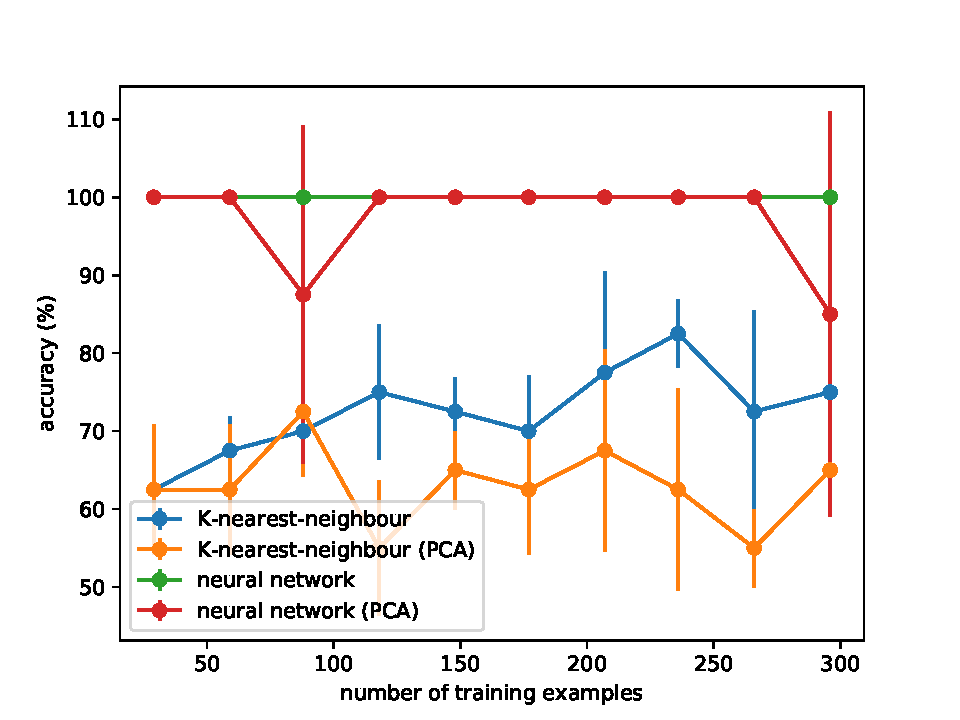
\includegraphics[scale=0.8,angle=0,trim=0cm 0cm 0.0cm 0cm]{fig_accuracy.pdf}
\caption{Percentage of correctly-classified samples in the test data vs the number of samples in the training data. The colours indicate whether a K-nearest-neighbour method or neural network approach was used to classify the dataset, and whether PCA was first used to collapse the 4D data space to a 2D dataspace.}
\label{fig_accuracy}
\end{figure}


\begin{figure}
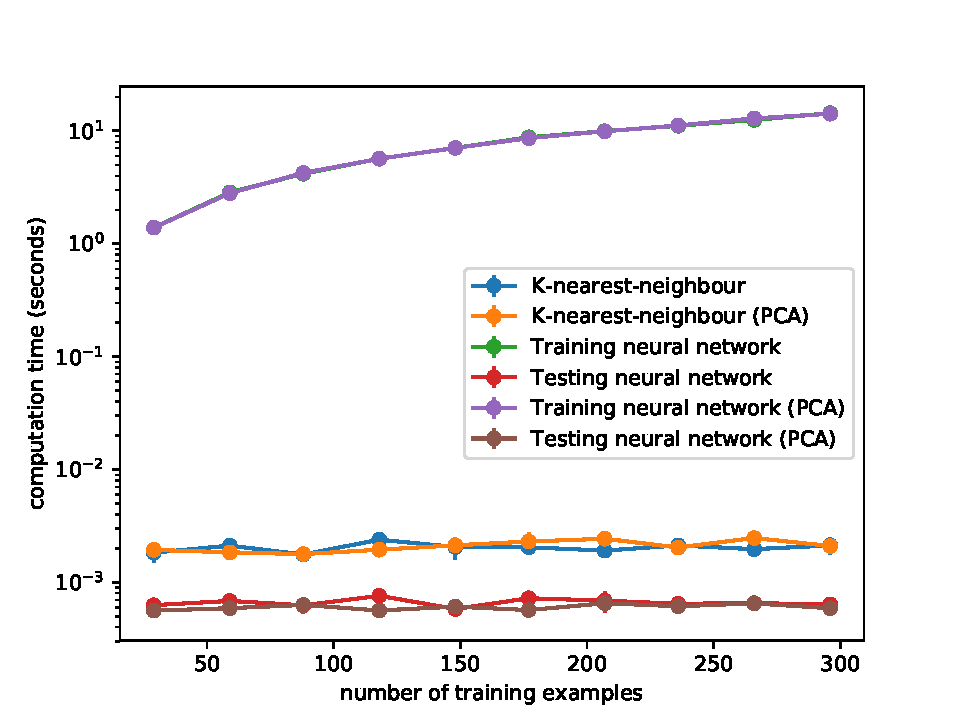
\includegraphics[scale=0.8,angle=0,trim=0cm 0cm 0.0cm 0cm]{fig_computetime.pdf}
\caption{Computation time (in seconds) as a functino of number of samples in the training data. The colours indicate whether a K-nearest-neighbour method or neural network approach was used to classify the dataset, and whether PCA was first used to collapse the 4D data space to a 2D dataspace.}
\label{fig_time}
\end{figure}


\section{Conclusions}
The main findings of the breast cancer classification study are as follows.

\begin{enumerate}
\item Both neural networks and K-nearest-neighbour algorithms accurately predict the survival rates for breast cancer as a function of four input markers .

\item The neural network consistently outperforms K-nearest neighbour for this data set and consistently achieving almost 100\% accuracy in comparison with the 70\% to 80\% observed with K-nearest neighbour.

\item Once trained the neural network also slightly outperformed K-nearest neighbour for computation speed, achieving millisecond performance. The dominant contributor to the neural net computation time was the training step. Though these algorithms tend to be pre-trained in a prototype phase for example before distribution as apps for use on smaller, lower powered devices. 
\end{enumerate}



Further comparison studies are forthcoming including a comparison between the two classification methods here and a random forest decision tree approach that will be introduced and used to classify data from an underwater sonar system intending to distinguish mines from background debris. This will be a different challenge than the breast cancer data set here as the sonar data includes 60 input attributes, presenting a much more challenging 60 dimensional parameter space to map. The results of this study and further projects can be found in the git hub link \footnote{href{ https://github.com/dstarkey23/projects}{\textcolor{blue}{https://github.com/dstarkey23/projects}}}. Thank you for your attention.



\end{document}



